% !TeX program = xelatex
\ifdefined\BookMaster\else
\documentclass[11pt,oneside]{article}
% !TeX program = xelatex
\usepackage[b5paper,left=22mm,right=22mm,top=20mm,bottom=22mm,footskip=11mm]{geometry}
\usepackage{fontspec}
\setmainfont{TeX Gyre Termes}
\setsansfont{TeX Gyre Heros}
\usepackage{amsmath,amssymb,mathtools,amsthm}
\renewcommand{\cdots}{\mathinner{\cdotp\cdotp\cdotp}}
\usepackage{graphicx,adjustbox,array,booktabs,longtable,multirow,enumitem,changepage,needspace}
\usepackage[table]{xcolor}
\usepackage{fancyhdr}
\raggedbottom
\interfootnotelinepenalty=10000
\newcommand{\BookFootnote}[2]{\begingroup\renewcommand{\thefootnote}{\fnsymbol{footnote}}\footnote[#1]{#2}\endgroup}
\newcommand{\BookFootnoteMark}[1]{\begingroup\renewcommand{\thefootnote}{\fnsymbol{footnote}}\footnotemark[#1]\endgroup}
\newcommand{\BookFootnoteText}[2]{\begingroup\renewcommand{\thefootnote}{\fnsymbol{footnote}}\footnotetext[#1]{#2}\endgroup}
\newenvironment{BookFloat}[1]{\par\addvspace{.6\baselineskip}\noindent\def\BookFloatID{#1}\begin{minipage}{\linewidth}\phantomsection\label{bookfloat:#1:start}}{\phantomsection\label{bookfloat:\BookFloatID:end}\end{minipage}\par\addvspace{.6\baselineskip}}

\usepackage[unicode,hidelinks]{hyperref}
\pagestyle{fancy}
\fancyhf{}
\newcommand{\BookFooter}{}
\fancyfoot[L]{\parbox[b]{\dimexpr\textwidth-15mm}{\footnotesize\BookFooter}}
\fancyfoot[R]{\footnotesize\thepage}
\renewcommand{\headrulewidth}{0pt}
\renewcommand{\footrulewidth}{0pt}
\setlength{\parindent}{0pt}
\setlength{\parskip}{0.2em}
\setlength{\emergencystretch}{3em}
\setlist{nosep,leftmargin=1.7em,labelsep=.65em}
\newif\ifBookNarrative
\BookNarrativetrue
\newenvironment{BookBody}{\setlength{\parindent}{0pt}}{}
\newcommand{\BookStatement}[1]{\par\addvspace{.6\baselineskip}\noindent #1\enspace\ignorespaces}
\newcommand{\BookLabel}[1]{\par\addvspace{.6\baselineskip}\needspace{3\baselineskip}\noindent\textbf{#1}\quad\ignorespaces}
\newcommand{\BookHeading}[1]{\par\addvspace{\baselineskip}\needspace{4\baselineskip}\noindent{\large\bfseries #1}\par\medskip}
\newcommand{\BookSubheading}[1]{\par\addvspace{.7\baselineskip}\needspace{3\baselineskip}\noindent{\bfseries #1}\par\smallskip}
\newcommand{\BookTextHeading}[1]{\par\addvspace{.7\baselineskip}\needspace{3\baselineskip}\noindent #1\par\smallskip}
\newcommand{\BookSectionTitle}[2]{\par\addvspace{1.2\baselineskip}\needspace{5\baselineskip}\noindent\colorbox{gray!25}{\sffamily\bfseries\small SECTION #1}\quad{\large\bfseries #2}\par\medskip}
\newcommand{\BookExerciseTitle}[1]{\par\addvspace{\baselineskip}\needspace{4\baselineskip}\noindent{\color{gray}\rule{1.5mm}{1.5mm}}\enspace{\large\bfseries Exercises #1}\par\medskip}
\newcommand{\BookBullet}[1]{\begin{list}{\textbullet}{\setlength{\leftmargin}{1.7em}\setlength{\labelwidth}{1em}\setlength{\labelsep}{.7em}\setlength{\topsep}{0pt}\setlength{\parsep}{0pt}\setlength{\itemsep}{0pt}}\item #1\end{list}}
\newcommand{\BookExercise}[2]{\begin{list}{\textbf{#1}}{\setlength{\leftmargin}{2.2em}\setlength{\labelwidth}{1.5em}\setlength{\labelsep}{.7em}\setlength{\topsep}{.15em}\setlength{\parsep}{0pt}\setlength{\itemsep}{0pt}}\item #2\end{list}}
\newcommand{\BookEnd}[1]{\unskip\nobreak\hfill\ensuremath{#1}}
\newcommand{\BookSource}[2]{\phantomsection\label{sourcepage:#1}} % Source-page anchors, retained through reflow.
\usepackage{multicol}
\usepackage{tikz}
\newcommand{\BookPartEntry}[2]{\par\noindent\makebox[17mm][l]{\bfseries Section #1}#2\par}
\newcommand{\BookPartTitle}[3]{\par\bigskip\noindent\begin{tikzpicture}\node[anchor=north west,inner sep=0pt,outer sep=0pt] (bookpart) at (0,0) {\begin{minipage}{\dimexpr\linewidth-.5pt}\hspace*{26mm}\begin{minipage}[t]{\dimexpr\linewidth-26mm}\begin{adjustbox}{max width=\linewidth}{\fontsize{20}{24}\selectfont\bfseries #2}\end{adjustbox}\par\vspace{6mm}\hrule\vspace{6mm}{\sffamily\footnotesize\setlength{\parskip}{.3em}#3}\vspace{3mm}\end{minipage}\end{minipage}};\path[shade,top color=gray!60,bottom color=white] (0,0) rectangle ([xshift=24mm]bookpart.south west);\node[anchor=north,font=\sffamily\bfseries\small] at (12mm,-2mm) {PART};\node[anchor=north,font=\sffamily\bfseries\Huge] at (12mm,-7mm) {#1};\end{tikzpicture}\par\bigskip}
\newsavebox{\BookMathBox}
\makeatletter
\newcommand{\BookInline}[1]{\leavevmode\hskip0pt\relax\begingroup\in@{\begin}{#1}\ifin@\sbox{\BookMathBox}{\(#1\)}\ifdim\wd\BookMathBox>\dimexpr\linewidth-1em\relax\resizebox{\dimexpr\linewidth-1em\relax}{!}{\usebox{\BookMathBox}}\else\(#1\)\fi\else\in@{\left}{#1}\ifin@\sbox{\BookMathBox}{\(#1\)}\ifdim\wd\BookMathBox>\dimexpr\linewidth-1em\relax\resizebox{\dimexpr\linewidth-1em\relax}{!}{\usebox{\BookMathBox}}\else\(#1\)\fi\else\(#1\)\fi\fi\endgroup\hskip0pt\relax}
\makeatother
\DeclareMathOperator{\Aut}{Aut}
\DeclareMathOperator{\End}{End}
\DeclareMathOperator{\Hom}{Hom}
\DeclareMathOperator{\GF}{GF}
\DeclareMathOperator{\irr}{irr}
\DeclareMathOperator{\lt}{lt}
\DeclareMathOperator{\lp}{lp}
\providecommand{\textcircled}[1]{\textnormal{(#1)}}

\begin{document}
\fi
\renewcommand{\BookFooter}{Section 20 Free Groups}
\pdfbookmark[0]{Section 20 Free Groups}{20_free_groups}
\ifdefined\BookMaster\else\setcounter{page}{172}\fi
% Source PDF page 189; original printed page 172
\BookSource{189}{172}
\BookNarrativetrue

\begin{BookBody}

\BookSectionTitle{20}{Free Groups}

\noindent For any group with elements \BookInline{a} and \BookInline{b} we have certain relations that \BookInline{a} and \BookInline{b} must satisfy simply because they are elements of a group. For example\BookInline{,\allowbreak a^{n}a^{m}= a^{n+ m}} and \BookInline{(ab)^{- 1}= } \BookInline{b^{- 1}a^{- 1}.} For most of the groups we have studied so far there are relations among the elements other than the relations that all groups possess. For example, the elements \BookInline{\mu } and \BookInline{\rho } in the dihedral group \BookInline{D_{n}} satisfy relations \BookInline{\rho \mu = \mu \rho ^{- 1}} and \BookInline{\mu ^{2}= \rho ^{n}= \iota.} In this section, we construct free groups that have only the relations that are required in the definition of a group. These groups and their factor groups as described in Section 21 are of great interest in the study of algebra and topology.

\BookTextHeading{\textbf{Words and Reduced Words}  }

\noindent Let \BookInline{A\neq } ø be any (not necessarily finite) set of elements \BookInline{a_{i}} for \BookInline{i\in I.} We think of \BookInline{A} as an\textbf{ alphabet} and of the \BookInline{a_{i}} as\textbf{ letters} in the alphabet. Any symbol of the form \BookInline{a}\textit{in} with \BookInline{n\in \mathbb{Z}} is a\textbf{ syllable} and a finite string \BookInline{w} of syllables written in juxtaposition is a\textbf{ word.} We also introduce the\textbf{ empty word} 1, which has no syllables.

\BookLabel{20.1 Example} Let \BookInline{A= \{a_{1},\allowbreak a_{2},\allowbreak a_{3}\}.} Then

\begin{center}\begin{adjustbox}{max width=\linewidth}\BookInline{\displaystyle a_{1}a_{3}^{- 4}a_{2}^{2}a_{3},\allowbreak a_{2}^{3}a_{2}^{- 1}a_{3}a_{1}^{2}a_{1}^{- 7},\allowbreak \;\text{and}\;a_{3}^{2}}\end{adjustbox}\end{center}

\noindent are all words, if we follow the convention of understanding that \BookInline{a_{i}^{1}} is the same as \BookInline{a_{i}.} \BookEnd{\blacktriangle}

\end{BookBody}

% Source PDF page 190; original printed page 173
\BookSource{190}{173}
\BookNarrativetrue

\begin{BookBody}

There are two natural types of modifications of certain words, the\textbf{ elementary con}\textbf{tractions.} The first type consists of replacing an occurrence of \BookInline{a}\textit{im}\BookInline{a}\textit{in} in a word by \BookInline{a}\textit{im}\BookInline{+ n.} The second type consists of replacing an occurrence of \BookInline{a_{i}^{0}} in a word by 1, that is, dropping it out of the word. By means of a finite number of elementary contractions, every word can be changed to a\textbf{ reduced word,} one for which no more elementary contractions are possible. Note that these elementary contractions formally amount to the usual manipulations of integer exponents and would have to be satisfied if we wish for the letters to be elements of a group.

\begin{center}\begin{adjustbox}{max width=\linewidth}\BookInline{\displaystyle a_{2}^{3}a_{2}^{- 1}a_{3}a_{1}^{2}a_{1}^{- 7}}\end{adjustbox}\end{center}

\begin{center}\begin{adjustbox}{max width=\linewidth}\BookInline{\displaystyle a_{2}^{2}a_{3}a_{1}^{- 5}}\end{adjustbox}\end{center}

\BookLabel{20.2 Example} The reduced form of the word of Example 20.1 is. \BookEnd{\blacktriangle}

It should be said here once and for all that we are going to gloss over several points that some books spend pages proving, usually by complicated induction arguments broken down into many cases. For example, suppose we are given a word and wish to find its reduced form. There may be a variety of elementary contractions that could be performed first. How do we know that the reduced word we end up with is the same no matter in what order we perform the elementary contractions? The student will probably say this is obvious. Some authors spend considerable effort proving this. The authors agree here with the student. Proofs of this sort we regard as tedious, and they have never made us more comfortable about the situation. However, the authors are the first to acknowledge that we are not great mathematicians. In deference to the fact that many mathematicians feel that these things do need considerable discussion, we shall mark an occasion when we just state such facts by the phrase, “It would seem obvious that,” keeping the quotation marks.

\BookTextHeading{\textbf{Free Groups}  }

\noindent Let the set of all reduced words formed from our alphabet \BookInline{A} be \BookInline{F[A].} We now make \BookInline{F[A]} into a group in a natural way. For \BookInline{w_{1}} and \BookInline{w_{2}} in \BookInline{F[A],\allowbreak } define \BookInline{w_{1}\cdot w_{2}} to be the reduced form of the word obtained by the juxtaposition \BookInline{w_{1}w_{2}} of the two words.

\BookLabel{20.3 Example} If

\begin{center}\begin{adjustbox}{max width=\linewidth}\BookInline{\displaystyle w_{1}= a_{2}^{3}a_{1}^{- 5}a_{3}^{2}}\end{adjustbox}\end{center}

\noindent and

\begin{center}\begin{adjustbox}{max width=\linewidth}\BookInline{\displaystyle w_{2}= a_{3}^{- 2}a_{1}^{2}a_{3}a_{2}^{- 2},\allowbreak }\end{adjustbox}\end{center}

\noindent then \BookInline{w_{1}\cdot w_{2}= a_{2}^{3}a_{1}^{- 3}a_{3}a_{2}^{- 2}.} \BookEnd{\blacktriangle}

“It would seem obvious that” this operation of multiplication on \BookInline{F[A]} is well defined and associative. The empty word 1 acts as an identity element. “It would seem obvious that” given a reduced word \BookInline{w\in F[A],\allowbreak } if we form the word obtained by first writing the syllables of \BookInline{w} in the opposite order and second by replacing each \BookInline{a}\textit{in} by \BookInline{a_{i}^{- n},\allowbreak } then the resulting word \BookInline{w^{- 1}} is a reduced word also, and

\begin{center}\begin{adjustbox}{max width=\linewidth}\BookInline{\displaystyle w\cdot w^{- 1}= w^{- 1}\cdot w= 1.}\end{adjustbox}\end{center}

\BookLabel{20.4 Definition} The group \BookInline{F[A]} just described is the\textbf{ free group generated} by \BookInline{A.} \BookEnd{\blacksquare}

Look back at Theorem 7.7 and the definition preceding it to see that the present use of the term\textit{ generated} is consistent with the earlier use.

Starting with a group \BookInline{G} and a generating set \BookInline{\{a_{i}\mid i\in I\},\allowbreak } which we will abbreviate by \BookInline{\{a_{i}\},\allowbreak } we might ask if \BookInline{G} is\textit{ free} on \BookInline{\{a_{i}\},\allowbreak } that is, if \BookInline{G} is essentially the free group generated by \BookInline{\{a_{i}\}.} We define precisely what this is to mean.

\end{BookBody}

% Source PDF page 191; original printed page 174
\BookSource{191}{174}
\BookNarrativetrue

\begin{BookBody}

\BookLabel{20.5 Definition} If \BookInline{G} is a group with a set \BookInline{A= \{a_{i}\}} of generators, and if \BookInline{G} is isomorphic to \BookInline{F[A]} under a map \BookInline{\phi:G\to F[A]} such that \BookInline{\phi (a_{i})= a_{i},\allowbreak } then \BookInline{G} is\textbf{ free on} \BookInline{A,\allowbreak } and the \BookInline{a_{i}} are\textbf{ free} \textbf{generators of} \BookInline{G.} A group is\textbf{ free} if it is free on some nonempty set \BookInline{A.}\BookEnd{\blacksquare}

\BookLabel{20.6 Example} The only example of a free group that has occurred before is \BookInline{\mathbb{Z},\allowbreak } which is free on one generator. Note that every free group is infinite, for it contains a subgroup isomorphic with \BookInline{\mathbb{Z}.}\BookEnd{\blacktriangle}

Refer to the literature for proofs of the next three theorems. We will not use these results. They are stated simply to inform us of these interesting facts.

\BookLabel{20.7 Theorem} If a group \BookInline{G} is free on \BookInline{A} and also on \BookInline{B,\allowbreak } then the sets \BookInline{A} and \BookInline{B} have the same number of elements; that is, any two sets of free generators of a free group have the same cardinality.

\BookLabel{20.8 Definition} If \BookInline{G} is free on \BookInline{A,\allowbreak } the number of elements in \BookInline{A} is the\textbf{ rank of the free group} \BookInline{G.\blacksquare } Actually, the next theorem is quite evident from Theorem 20.7.

\BookLabel{20.9 Theorem} Two free groups are isomorphic if and only if they have the same rank.

\BookLabel{20.10 Theorem} A nontrivial subgroup of a free group is free.

\BookLabel{20.11 Example} Let \BookInline{F[\{x,\allowbreak y\}]} be the free group on \BookInline{\{x,\allowbreak y\}.} Let

\begin{center}\begin{adjustbox}{max width=\linewidth}\BookInline{\displaystyle y_{k}= x^{k}yx^{- k}}\end{adjustbox}\end{center}

\noindent for \BookInline{k\geq 0.} The \BookInline{y_{k}} for \BookInline{k\geq 0} are free generators for the subgroup of \BookInline{F[\{x,\allowbreak y\}]} that they generate. This illustrates the bizarre fact that although a subgroup of a free group is free, the rank of the subgroup may be much greater than the rank of the whole group! \BookEnd{\blacktriangle}

\BookTextHeading{\textbf{Homomorphisms of Free Groups}  }

\noindent Our work in this section will be concerned primarily with homomorphisms defined on a free group. The results here are simple and elegant.

\BookLabel{20.12 Theorem} Let \BookInline{G} be generated by \BookInline{A= \{a_{i}\mid i\in I\}} and let \BookInline{G^{\prime }} be any group. If \BookInline{a_{i}^{\prime }} for \BookInline{i\in I} are any elements in \BookInline{G^{\prime },\allowbreak } not necessarily distinct, then there is at most one homomorphism \BookInline{\phi:G\to G^{\prime }} such that \BookInline{\phi (a_{i})= a_{i}^{\prime }.} If \BookInline{G} is free on \BookInline{A,\allowbreak } then there is exactly one such homomorphism.

\BookLabel{\textit{Proof}} Let \BookInline{\phi } be a homomorphism from \BookInline{G} into \BookInline{G^{\prime }} such that \BookInline{\phi (a_{i})= a_{i}^{\prime }.} Now by Theorem 7.7, for any \BookInline{x\in G} we have

\begin{center}\begin{adjustbox}{max width=\linewidth}\BookInline{\displaystyle x= \prod _{j}a_{i_{j}}^{n_{j}}}\end{adjustbox}\end{center}

\noindent for some finite product of the generators \BookInline{a_{i},\allowbreak } where the \BookInline{a_{i_{j}}} appearing in the product need not be distinct. Then since \BookInline{\phi } is a homomorphism, we must have

\begin{center}\begin{adjustbox}{max width=\linewidth}\BookInline{\displaystyle \phi (x)= \prod _{j}\phi \Big(a_{i_{j}}^{n_{j}}\Big)= \prod _{j}\Big(\mathrm{a}_{i_{j}}^{\prime }\Big)^{n_{j}}.}\end{adjustbox}\end{center}

\noindent Thus a homomorphism is completely determined by its values on elements of a generating set. This shows that there is at most one homomorphism such that \BookInline{\phi (a_{i})= a_{i}^{\prime }.}

\end{BookBody}

% Source PDF page 192; original printed page 175
\BookSource{192}{175}
\BookNarrativetrue

\begin{BookBody}

Now suppose \BookInline{G} is free on \BookInline{A;} that is\BookInline{,\allowbreak G= F[A].} For

\begin{center}\begin{adjustbox}{max width=\linewidth}\BookInline{\displaystyle x= \prod _{j}a_{i_{j}}^{n_{j}}}\end{adjustbox}\end{center}

\noindent in \BookInline{G,\allowbreak } define \BookInline{\psi:G\to G^{\prime }} by

\begin{center}\begin{adjustbox}{max width=\linewidth}\BookInline{\displaystyle \psi (x)= \prod _{j}\Big(a_{i_{j}}^{\prime }\Big)^{n_{j}}.}\end{adjustbox}\end{center}

\noindent The map is well defined, since \BookInline{F[A]} consists precisely of reduced words; no two different formal products in \BookInline{F[A]} are equal. Since the rules for computation involving exponents in \BookInline{G^{\prime }} are formally the same as those involving exponents in \BookInline{G,\allowbreak } it is clear that \BookInline{\psi (xy)= \psi (x)\psi (y)} for any elements \BookInline{x} and \BookInline{y} in \BookInline{G,\allowbreak } so \BookInline{\psi } is indeed a homomorphism\BookInline{.}\BookEnd{\blacklozenge}

Perhaps we should have proved the first part of Theorem 20.12 earlier, rather than having relegated it to the exercises. Note that the theorem states that \BookInline{a} \textit{homomorphism of} \BookInline{a} \textit{group is completely determined if we know its value on each element of} \BookInline{a} \textit{generating} \textit{set}. In particular, a homomorphism of a cyclic group is completely determined by its value on any single generator of the group.

\BookLabel{20.13 Theorem} Every group \BookInline{G^{\prime }} is a homomorphic image of a free group \BookInline{G.}

\BookLabel{\textit{Proof}} Let \BookInline{G^{\prime }= \{a_{i}^{\prime }\mid i\in I\},\allowbreak } and let \BookInline{A= \{a_{i}\mid i\in I\}} be a set with the same number of elements as \BookInline{G^{\prime }.} Let \BookInline{G= F[A].} Then by Theorem 20.12 there exists a homomorphism \BookInline{\psi } mapping \BookInline{G} into \BookInline{G^{\prime }} such that \BookInline{\psi (a_{i})= a_{i}^{\prime }.} Clearly the image of \BookInline{G} under \BookInline{\psi } is all of \BookInline{G^{\prime }.}\BookEnd{\blacklozenge}

\BookTextHeading{\textbf{Another Look at Free Abelian Groups}  }

\noindent It is important that we do not confuse the notion of a free group with the notion of a free abelian group. A free group on more than one generator is not abelian. In the preceding section, we defined a free abelian group as an abelian group that has a basis, that is, a generating set satisfying properties described in Theorem 19.1. There is another approach, via free groups, to free abelian groups. We now describe this approach.

Let \BookInline{F[A]} be the free group on the generating set \BookInline{A.} We shall write \BookInline{F} in place of \BookInline{F[A]} for the moment. Note that \BookInline{F} is not abelian if \BookInline{A} contains more than one element. Let \BookInline{C} be the commutator subgroup of \BookInline{F.} Then \BookInline{F/C} is an abelian group, and it is not hard to show that \BookInline{F/C} is free abelian with basis \BookInline{\{}\textit{aC} \BookInline{\mid a\in A\}.} If\textit{ aC} is renamed \BookInline{a,\allowbreak } we can view \BookInline{F/C} as a free abelian group with basis \BookInline{A.} This indicates how a free abelian group having a given set as basis can be constructed. Every free abelian group can be constructed in this fashion, up to isomorphism. That is, if \BookInline{G} is free abelian with basis \BookInline{X,\allowbreak } form the free group \BookInline{F[X],\allowbreak } form the factor group of \BookInline{F[X]} modulo its commutator subgroup, and we have a group isomorphic to \BookInline{G.}

Theorems 20.7, 20.9, and 20.10 hold for free abelian groups as well as for free groups. In fact, the abelian version of Theorem 20.10 was proved for the finite rank case in Theorem 19.11. In contrast to Example 20.11 for free groups, it is true that for a free abelian group the rank of a subgroup is at most the rank of the entire group. Theorem 19.11 also showed this for the finite rank case.

\end{BookBody}

% Source PDF page 193; original printed page 176
\BookSource{193}{176}
\BookNarrativefalse

\begin{BookBody}

\BookExerciseTitle{20}

\BookTextHeading{\textbf{Computations}}

\BookExercise{1.}{Find the reduced form and the inverse of the reduced form of each of the following words. \textbf{a}\BookInline{.a^{2}b^{- 1}b^{3}a^{3}c^{- 1}c^{4}b^{- 2}} \textbf{b}\BookInline{.a^{2}a^{- 3}b^{3}a^{4}c^{4}c^{2}a^{- 1}}}

\BookExercise{2.}{Compute the products given in parts (a) and (b) of Exercise 1 in the case that \BookInline{\{a,\allowbreak b,\allowbreak c\}} is a set of generators forming a basis for a free abelian group. Find the inverse of these products.}

\BookExercise{3.}{How many different homomorphisms are there of a free group of rank 2 into \textbf{a}\BookInline{.\mathbb{Z}_{4}}? \textbf{b}\BookInline{.\mathbb{Z}_{6}}? \textbf{c}\BookInline{.S_{3}}?}

\BookExercise{4.}{How many different homomorphisms are there of a free group of rank 2 onto \textbf{a}\BookInline{.\mathbb{Z}_{4}}? \textbf{b}\BookInline{.\mathbb{Z}_{6}}? \textbf{c}\BookInline{.S_{3}}?}

\BookExercise{5.}{How many different homomorphisms are there of a free abelian group of rank 2 into \textbf{a}\BookInline{.\mathbb{Z}_{4}}? \textbf{b}\BookInline{.\mathbb{Z}_{6}}? \textbf{c}\BookInline{.S_{3}}?}

\BookExercise{6.}{How many different homomorphisms are there of a free abelian group of rank 2 onto \textbf{a}\BookInline{.\mathbb{Z}_{4}}? \textbf{b}\BookInline{.\mathbb{Z}_{6}}? \textbf{c}\BookInline{.S_{3}}?}

\BookTextHeading{\textbf{Concepts}}

\noindent In Exercises 7 and 8, correct the definition of the italicized term without reference to the text, if correction is needed, so that it is in a form acceptable for publication.

\BookExercise{7.}{A\textit{ reduced word} is one in which there are no appearances in juxtaposition of two syllables having the same letter and also no appearances of a syllable with exponent 0.}

\BookExercise{8.}{The\textit{ rank of} \BookInline{a} \textit{free group} is the number of elements in a set of generators for the group.}

\BookExercise{9.}{Take one of the instances in this section in which the phrase “It would seem obvious that” was used and discuss your reaction in that instance.}

\BookExercise{10.}{Determine whether each of the following is true or false.}

\BookExercise{a.}{Every proper subgroup of a free group is a free group.}

\BookExercise{b.}{Every proper subgroup of every free abelian group is a free group.}

\BookExercise{c.}{A homomorphic image of a free group is a free group.}

\BookExercise{d.}{Every free abelian group has a basis.}

\BookExercise{e.}{The free abelian groups of finite rank are precisely the finitely generated abelian groups.}

\BookExercise{f.}{No free group is free.}

\BookExercise{g.}{No free abelian group is free.}

\BookExercise{h.}{No free abelian group of rank \BookInline{>1} is free.}

\BookExercise{i.}{Any two free groups are isomorphic.}

\BookExercise{j.}{Any two free abelian groups of the same rank are isomorphic.}

\BookTextHeading{\textbf{Theory}}

\BookExercise{11.}{Let \BookInline{G} be a finitely generated abelian group with identity 0. A finite set \BookInline{\{b_{1},\allowbreak \cdots,\allowbreak b_{n}\},\allowbreak } where \BookInline{b_{i}\in G,\allowbreak } is a\textbf{ basis} \textbf{for} \BookInline{G} if \BookInline{\{b_{1},\allowbreak \cdots,\allowbreak b_{n}\}} generates \BookInline{G} and \BookInline{\sum _{i= 1}^{n}m_{i}b_{i}= 0\mathrm{i}} f and only if each \BookInline{m_{i}b_{i}= 0,\allowbreak } where \BookInline{m_{i}\in \mathbb{Z}.}}

\BookExercise{a.}{Show that \BookInline{\{2,\allowbreak 3\}} is not a basis for \BookInline{\mathbb{Z}_{4}.} Find a basis for \BookInline{\mathbb{Z}_{4}.}}

\BookExercise{b.}{Show that both \BookInline{\{1\}} and \BookInline{\{2,\allowbreak 3\}} are bases for \BookInline{\mathbb{Z}_{6}.(}This shows that for a finitely generated abelian group \BookInline{G} with torsion, the number of elements in a basis may vary; that is, it need not be an\textit{ invariant} of the group \BookInline{G.)}}

\BookExercise{c.}{Is a basis for a free abelian group as we defined it in Section 19 a basis in the sense in which it is used in this exercise?}

\BookExercise{d.}{Show that every finite abelian group has a basis \BookInline{\{b_{1},\allowbreak \cdots,\allowbreak b_{n}\},\allowbreak } where the order of \BookInline{b_{i}} divides the order of \BookInline{b_{i+ 1}.}}

\end{BookBody}

% Continuation on source PDF page 194, preceding Section 21
\BookNarrativefalse

\begin{BookBody}

\noindent In present-day expositions of algebra, a frequently used technique (particularly by the disciples of N. Bourbaki) for introducing a new algebraic entity is the following:

\BookExercise{1.}{Describe algebraic properties that this algebraic entity is to possess.}

\BookExercise{2.}{Prove that any two algebraic entities with these properties are isomorphic, that is, that these properties characterize the entity.}

\BookExercise{3.}{Show that at least one such entity exists.}

\noindent The next three exercises illustrate this technique for three algebraic entities, each of which we have met before. So that we do not give away their identities, we use fictitious names for them in the first two exercises. The last part of these first two exercises asks us to give the usual name for the entity.

\BookExercise{12.}{Let \BookInline{G} be any group. An abelian group \BookInline{G^{\ast }} is a\textbf{ blip group of} \BookInline{G} if there exists a fixed homomorphism \BookInline{\phi } of \BookInline{G} onto \BookInline{G^{\ast }} such that each homomorphism \BookInline{\psi } of \BookInline{G} into an abelian group \BookInline{G^{\prime }} can be factored as \BookInline{\psi = \theta \phi,\allowbreak } where \BookInline{\theta } is a homomorphism of \BookInline{G^{\ast }} into \BookInline{G^{\prime }(}see Fig. 20.14).}

\BookExercise{a.}{Show that any two blip groups of \BookInline{G} are isomorphic. [\textit{Hint:} Let \BookInline{G_{1}^{\ast }} and \BookInline{G_{2}^{\ast }} be two blip groups of \BookInline{G.} Then each of the fixed homomorphisms \BookInline{\phi _{1}:G\to G_{1}^{\ast }} and \BookInline{\phi _{2}:G\to G_{2}^{\ast }} can be factored via the other blip group according to the definition of a blip group; that is\BookInline{,\allowbreak \phi _{1}= \theta _{1}\phi _{2}} and \BookInline{\phi _{2}= \theta _{2}\phi _{1}.} Show that \BookInline{\theta _{1}} is an isomorphism of \BookInline{G_{2}^{\ast }} onto \BookInline{G_{1}^{\ast }} by showing that both \BookInline{\theta _{1}\theta _{2}} and \BookInline{\theta _{2}\theta _{1}} are identity maps.]}

\BookExercise{b.}{Show for every group \BookInline{G} that a blip group \BookInline{G^{\ast }} of \BookInline{G} exists.}

\BookExercise{c.}{What concept that we have introduced before corresponds to this idea of a blip group of \BookInline{G}?}

\begin{BookFloat}{20_free_groups-p194-9}
\begin{center}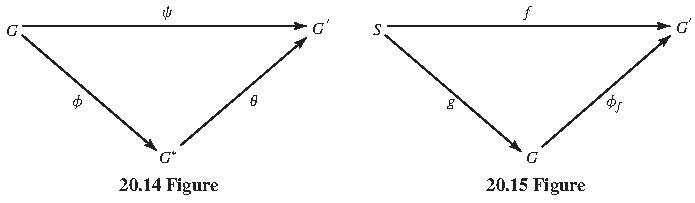
\includegraphics[width=0.953\linewidth,height=.8\textheight,keepaspectratio]{assets/p194_00.pdf}\end{center}
\end{BookFloat}

\BookExercise{13.}{Let \BookInline{S} be any set. A group \BookInline{G} together with a fixed function \BookInline{g:S\to G} constitutes a\textbf{ blop group on} \BookInline{S} if for each group \BookInline{G^{\prime }} and map \BookInline{f:S\to G^{\prime }} there exists a\textit{ unique} homomorphism \BookInline{\phi _{f}} of \BookInline{G} into \BookInline{G^{\prime }} such that \BookInline{f= \phi _{f}g(}see Fig. 20.15).}

\BookExercise{a.}{Let S be a fixed set. Show that if both \BookInline{G_{1},\allowbreak } together with \BookInline{g_{1}:S\to G_{1},\allowbreak } and \BookInline{G_{2},\allowbreak } together with \BookInline{g_{2}:S\to G_{2},\allowbreak } are blop groups on \BookInline{S,\allowbreak } then \BookInline{G_{1}} and \BookInline{G_{2}} are isomorphic. [\textit{Hint:} Show that \BookInline{g_{1}} and \BookInline{g_{2}} are one-to-one maps and that \BookInline{g_{1}S} and \BookInline{g_{2}S} generate \BookInline{G_{1}} and \BookInline{G_{2},\allowbreak } respectively. Then proceed in a way analogous to that given by the hint for Exercise 12.]}

\BookExercise{b.}{Let \BookInline{S} be a set. Show that a blop group on \BookInline{S} exists. You may use any theorems of the text.}

\BookExercise{c.}{What concept that we have introduced before corresponds to this idea of a blop group on \BookInline{S}?}

\BookExercise{14.}{Characterize a free abelian group by properties in a fashion similar to that used in Exercise 13.}

\end{BookBody}
\ifdefined\BookMaster\let\BookFinish\relax\else\def\BookFinish{\end{document}}\fi\BookFinish
